\documentclass{article}

\usepackage[T1]{fontenc}
\usepackage{fullpage}
\usepackage{xcolor}
\usepackage[parfill]{parskip}
\usepackage{bm}
\usepackage{xspace}
\usepackage{graphicx}
% \usepackage{amsmath}
% \usepackage{amssymb}
\usepackage{url}

\title{Formalización de la propiedad de Progreso\\para el \stlcw}
  % \\[1ex]{\LARGE Avances}}
% \subtitle{Blueprint}
\author{Cristian Sottile}
\date{20 de octubre de 2023}

\newcommand{\stlcw}{$\lambda-$cálculo simplemente tipado\xspace}
\newcommand{\stlc}{$\lambda^{\rightarrow}$}
\newcommand{\lamg}{\ensuremath{\lambda^{\mathbb{m}}}\xspace}
\newcommand{\lamm}{\ensuremath{\lambda^{\mathbb{m}}}\xspace}
\newcommand{\wme}{\ensuremath{\mathcal{W}}\xspace}
\newcommand{\wmem}[1]{\ensuremath{\mathcal{W}(#1)}\xspace}
\newcommand{\tmme}{\ensuremath{\mathcal{T}^{\mathbb{m}}}\xspace}
\newcommand{\tmmem}[1][M]{\ensuremath{\mathcal{T}^{\mathbb{m}}(#1)}\xspace}
\newcommand{\tme}{\ensuremath{\mathcal{T}}\xspace}
\newcommand{\tmem}[1][M]{\ensuremath{\mathcal{T}(#1)}\xspace}
\newcommand{\tom}{\ensuremath{\rightarrow_m}\xspace}
\newcommand{\tob}{\ensuremath{\rightarrow_{\beta}}\xspace}
\newcommand{\tof}{\ensuremath{\triangleright}\xspace}
\newcommand{\wrap}[1]{\ensuremath{\bm{\{}#1\bm{\}}}\xspace}
\newcommand{\wei}[1]{\ensuremath{\mathsf{w}(#1)}\xspace}
\newcommand{\maxdeg}[1]{\ensuremath{\dh(#1)}\xspace}
\newcommand{\simp}[1]{\ensuremath{\mathsf{S}_*(#1)}\xspace}
\newcommand{\simpd}[2][d]{\ensuremath{\mathsf{S}_{#1}(#2)}\xspace}

\newcommand{\inte}[1]{\ensuremath{[[#1]]}}
\newcommand{\lam}[2][x]{\ensuremath{\lambda #1 . #2}}

\newcommand{\sep}{\ensuremath{\ |\ }}
\newcommand{\ie}{{\em i.e.}\xspace}
\newcommand{\eg}{{\em e.g.}\xspace}
\newcommand{\ver}[1]{\textcolor{red}{#1}}

\newcommand{\n}[1]{\ensuremath{\mathsf{#1}}}

\begin{document}

\maketitle

% \begin{abstract}
%   La propuesta es formalizar la propiedad de Progreso del \stlcw. El objetivo del
%   trabajo es comprender en profundidad las maneras de formalizar el \stlcw y sus
%   propiedades principales. El asistente a usar será Agda por el mismo motivo,
%   comprender en profundidad esa herramienta en particular.
% \end{abstract}

\section{Avances}

En este mes estuve siguiendo el libro PLFA de Wadler para interiorizarme con el
asistente. Comparto el repositorio en el que estuve copiando las definiciones e
implementando los ejercicios propuestos. Estoy en el capítulo de
Cuantificadores, me quedan los capítulos de Decidibilidad y de Listas, y luego
planeo empezar con la implementación del $\lambda-$cálculo simplemente tipado
para poder probar la propiedad de progreso. No me topé con mayores dificultades
aprendiendo Agda. Sí fui anotando algunas dudas que aprovecho para copiar acá.

\section{Consultas}

\subsection{Ignorando parámetros sin éxito}

Aclaro que usé este formato inusual de definir las funciones en el
\texttt{where} solo para ver si funcionaba.

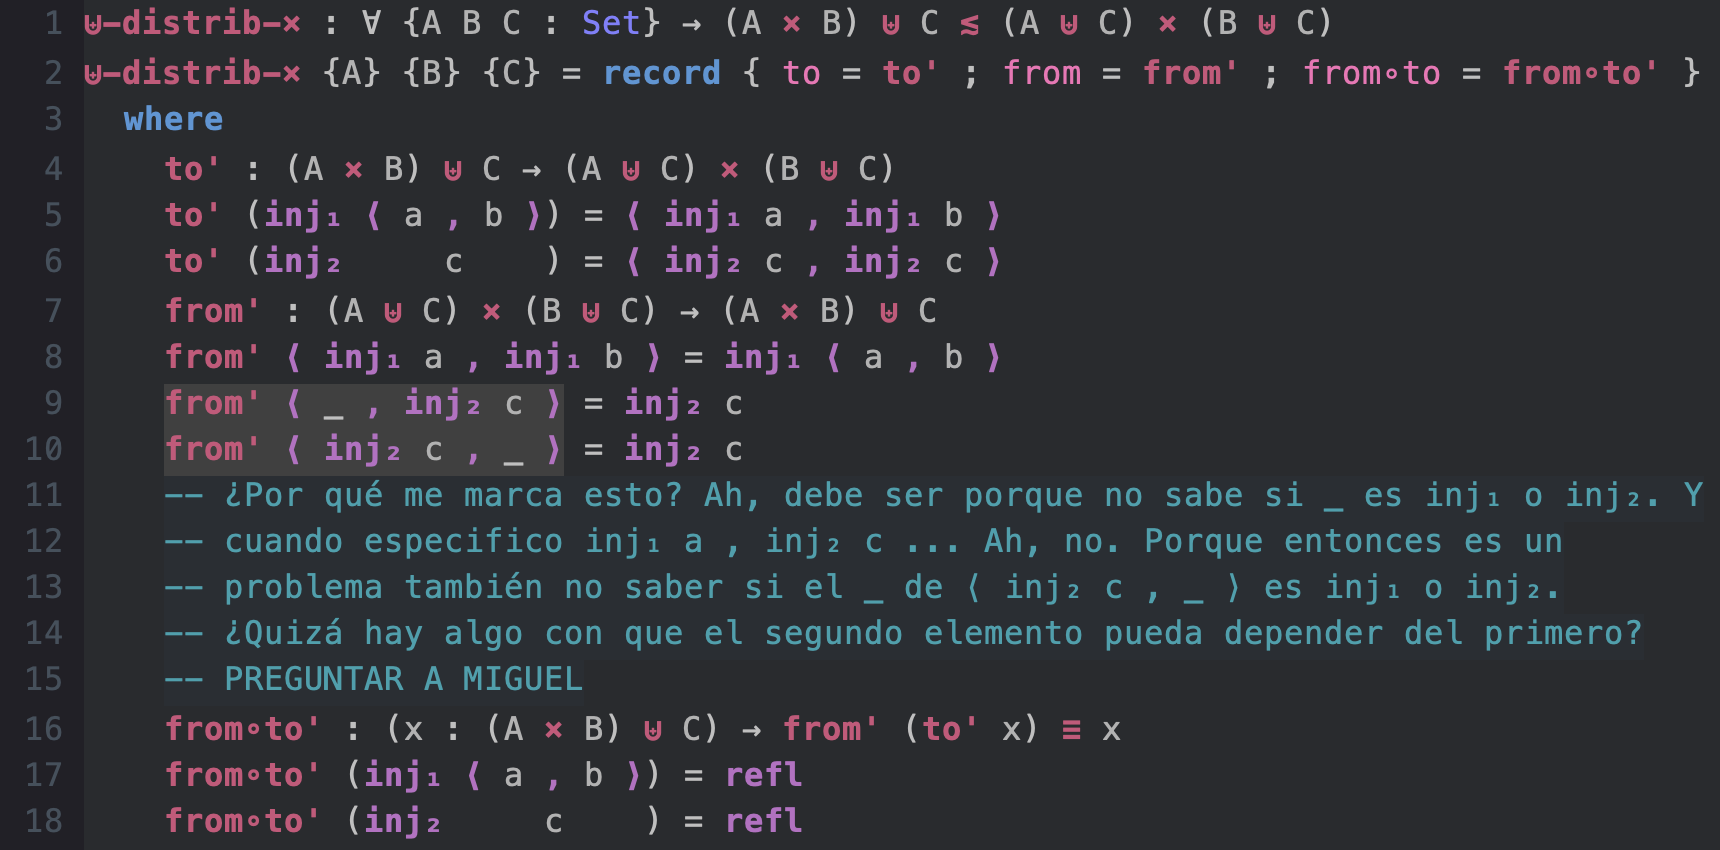
\includegraphics[width=\textwidth]{consulta2.png}

\subsection{Normalización de goals pero no de términos}

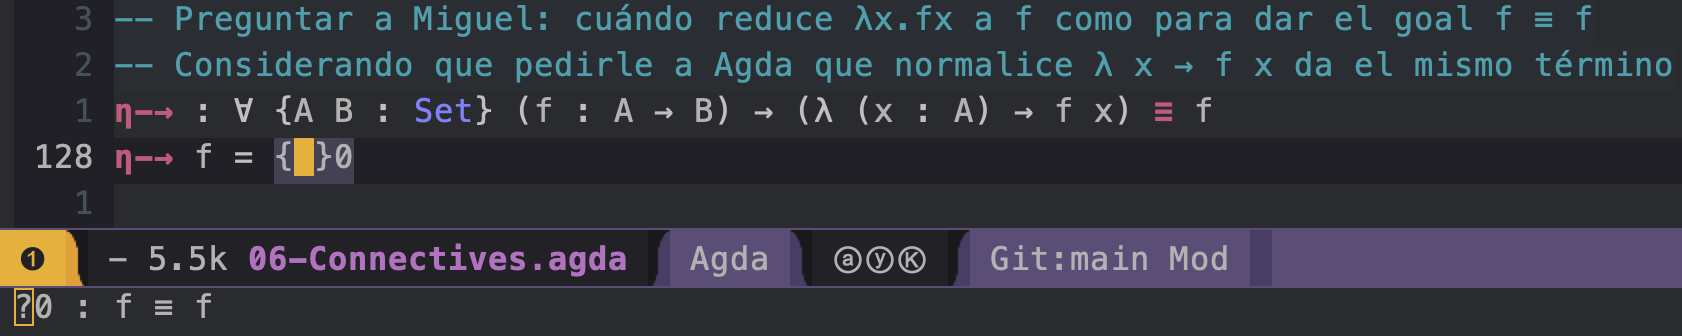
\includegraphics[width=\textwidth]{consulta1.png}


\end{document}